\section{Project Schedule}
Below is the Gantt chart of our project Schedule to perfrom these specific tasks between these time frames.
\begin{figure}[H]
    \centering
        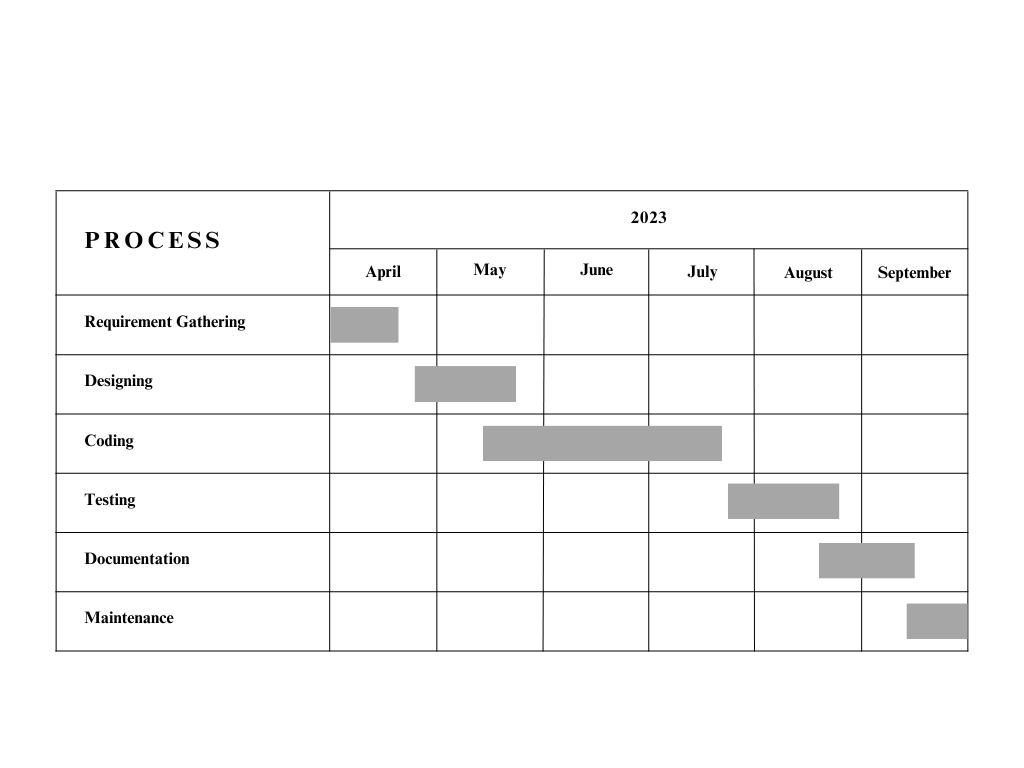
\includegraphics[width=400px]{Diagrams/Gantt_Chart.png}
    \caption{Gantt Chart of Schedule}
\end{figure}

\lstset{frame=tb,
  language=PHP,
  aboveskip=3mm,
  belowskip=3mm,
  showstringspaces=false,
  columns=flexible,
  basicstyle={\small\ttfamily},
  numbers=none,
  numberstyle=\tiny\color{gray},
  keywordstyle=\color{blue},
  commentstyle=\color{dkgreen},
  stringstyle=\color{mauve},
  breaklines=true,
  breakatwhitespace=true,
  tabsize=3
}
\section{Setup Guide to run Code Connect Locally}
\begin{enumerate}
    \item \textbf{Prerequisite:}
    \begin{enumerate}
        \item XAMPP
        \item Operating System that support XAMPP
        \item Internet Connection for CDN libraries.
        \item Project Files Cloned from Git Hub
    \end{enumerate}
    \item Clone Repo in htdocs/\\
    \begin{verbatim}
git clone https://github.com/sushantbramhacharya/CodeConnectBE.git
    \end{verbatim}
    Clone DB Repo in mysql/data\\
    \begin{verbatim}
git clone https://github.com/sushantbramhacharya/CodeConnectDB.git
    \end{verbatim}
    \item Open XAMPP Control Panel
    \item Start Apache and MySQL Servers
    \item Run it on http://localhost/ or codeConnect directory
\end{enumerate}

\section{MySQL Connection in our CodeConnect PHP}
\vspace{1cm}
\begin{lstlisting}
    <?php
    $servername = "localhost";
    $username = "root";
    $password = "";
    $dbname = "codeconnect";

    $conn = new mysqli($servername, $username, $password, $dbname);

    if ($conn->connect_error) {
        die("Connection failed: " . $conn->connect_error);
    }
    ?>
    \end{lstlisting}

\section{Supervisor Consultation Form}
\begin{figure}[H]
    \centering
        \includegraphics[width=400px]{Appendix/supervisor-form.jpg}
    \caption{Supervisor Consultation Form}
\end{figure}